\documentclass[12pt,a4paper]{report}

\usepackage[utf8]{inputenc} % pentru suport diacritice
\usepackage[romanian]{babel} % setări pentru limba română 
\renewcommand\familydefault{\sfdefault} % sans serif

\usepackage[margin=2.54cm]{geometry}	% dimensiuni pagină și margini
\usepackage{graphicx} % support the \includegraphics command and options

% formatting sections and subsections
\usepackage{listings}
\usepackage[section]{placeins}
\usepackage[ separate-uncertainty = true, multi-part-units = repeat]{siunitx}
\usepackage[nottoc,numbib]{tocbibind}
\usepackage{indentfirst}
\usepackage[parfill]{parskip}
\usepackage{textcase}
\usepackage[titletoc, title]{appendix}
\usepackage{titlesec}
\titleformat{\chapter}{\large\bfseries}{\thechapter}{2ex}{}[\vspace*{-1.5cm}]
\titleformat*{\section}{\large\bfseries}
\titleformat*{\subsection}{\large\bfseries}
\titleformat*{\subsubsection}{\large\bfseries}

\usepackage{chngcntr}
\counterwithout{figure}{chapter} % no chapter number in figure labels
\counterwithout{table}{chapter} % no chapter number in table labels
\counterwithout{equation}{chapter} % no chapter number in equation labels

\usepackage{booktabs} % for much better looking tables
\usepackage{url} % Useful for inserting web links nicely
\usepackage[bookmarks,unicode,hidelinks]{hyperref}

\usepackage{array} % for better arrays (eg matrices) in maths
\usepackage{paralist} % very flexible & customisable lists (eg. enumerate/itemize, etc.)
\usepackage{verbatim} % adds environment for commenting out blocks of text & for better verbatim
\usepackage{subfig} % make it possible to include more than one captioned figure/table in a single float
\usepackage{enumitem}
\setlist{noitemsep}

%%% HEADERS & FOOTERS
\usepackage{fancyhdr}
\pagestyle{empty}
\renewcommand{\headrulewidth}{0pt}
\renewcommand{\footrulewidth}{0pt}
\lhead{}\chead{}\rhead{}
\lfoot{}\cfoot{\thepage}\rfoot{}



\newcommand{\HeaderLineSpace}{-0.5cm}
\newcommand{\UniTextRO}{Universitatea POLITEHNICA București \\[\HeaderLineSpace] 
Facultatea Automatică și Calculatoare \\[\HeaderLineSpace]
Departamentul Automatică și Informatică Industrială\\}
\newcommand{\DiplomaRO}{LUCRARE DE LICENȚĂ}
\newcommand{\AdvisorRO}{Coordonator științific:}
\newcommand{\BucRO}{BUCUREȘTI}

\newcommand{\frontPage}[5]{
\begin{titlepage}
\begin{center}
{\Large #1}  % header (university, faculty, department)
\vspace{50pt}
\begin{tabular}{p{6cm}p{3cm}}

\includegraphics[scale=0.8]{pics/upb-logo.jpg} &
	
\includegraphics[scale=0.27,clip=true]{pics/acs_logo.jpg}
\end{tabular}

\vspace{105pt}
{\Huge #2}\\                           % diploma project text
\vspace{40pt}
{\Large #3}\\ \vspace{0pt}  % project title
\vspace{40pt}
{\LARGE \Name}\\                   % student name
\end{center}
\vspace{60pt}
\begin{tabular*}{\textwidth}{@{\extracolsep{\fill}}p{6cm}r}
&{\large\textbf{#4}}\vspace{10pt}\\      % scientific advisor
&{\large \Advisor}                                    % advisor name
\end{tabular*}
\vspace{20pt}
\begin{center}
{\large\textbf{#5}}\\                                % bucharest
\vspace{0pt}
{\normalsize \Year}
\end{center}
\end{titlepage}
}

\newcommand{\frontPageRO}{\frontPage{\UniTextRO}{\DiplomaRO}{\ProjectTitleRO}{\AdvisorRO}{\BucRO}}

\linespread{1.5}
\setlength\parindent{15pt}
\setlength\parskip{.28cm}

%% Abstract macro
\newcommand{\AbstractPage}{
\begin{titlepage}
\textbf{\large TODO:  SINOPSIS}\par
\AbstractRO\par\vfill
\end{titlepage}
}


%%%%%%%%%%%%%%%%%%%%%%%%%%%%%%%%%%%%%%%%%%%%%%%%%%   
%%
%%          End of template definitions
%%   
%%%%%%%%%%%%%%%%%%%%%%%%%%%%%%%%%%%%%%%%%%%%%%%%%%

\newcommand{\ProjectTitleRO}{Integrarea unei plăci de dezvoltare bazate pe microcontrolerul ATSAMR21 cu mediul de dezvoltare Arduino IDE}
\newcommand{\Name}{Blânzeanu Doru-Florin}
\newcommand{\Advisor}{SI. dr. ing. Radu Pietraru}
\newcommand{\Year}{2018}




% Setări document
\title{Proiect de diplomă}
\author{\Name}
\date{\Year}

\newcommand{\Thanks}{(opțional) Aici puteți introduce o secțiunea specială de mulțumiri / acknowledgments. }

\newcommand{\AbstractRO}{Sinopsisul proiectului are rol de introducere, conținând atât o descriere pe scurt a problemei abordate cât și o enumerare sumară a rezultatelor și a concluziilor. Se recomandă ca sinopsisul să fie redactat într-un limbaj accesibil unei persoane nefamiliarizate cu domeniul, dar în același timp destul de specific pentru a oferi rapid o vedere de ansamblu asupra proiectului prezentat.
Sinopsisul proiectului va fi redactat atât în română cât și în engleză. Ca dimensiunea recomandată aceasta secțiune va avea maxim 200 de cuvinte pentru fiecare variantă. Împreună, ambele variante se vor încadra într-o singură pagină.}

\begin{document}

\frontPageRO

%empty page
\clearpage
\thispagestyle{empty}
\phantom{a}
\vfill
\newpage
\vfill

\begingroup
\linespread{1}
\tableofcontents
\endgroup

%empty page
\clearpage
\thispagestyle{empty}
\phantom{a}
\vfill
\newpage
\vfill

\chapter{Introducere}\pagestyle{fancy}
În lucrarea de față se va vorbi despre integrarea unei noi plăci de dezvoltare, Atmel SAMR21 Xplained Pro, în ecosistemul Arduino. Deasemenea, se va face o analiză asupra domeniului Internetului Lucrurilor(IoT)\footnote{IoT = Internetul of Things} în care se utilizează microcontrolerul acestei placi de dezvoltare și a importanței circuitelor care îmbină puterea de calcul cu comunicația radio.

Pentru dezvoltarea de sisteme integrate exista opțiunea de a alege componenta de bază pentru procesare fie un microcontroler, fie un microprocesor. Ambele abordări au avantajele și dezavantajele lor, dar în general în aplicațiile în care contează dimensiunea, costul și puterea consumată, este preferat un microcontroler. Când vine vorba despre o aplicație care necesită comunicație radio, alegerea unui microcontroler care are integrată o componentă radio este mult mai convenabilă spre deosebire de un microcontroler care nu dispune de această componentă la care să se adauge componenta radio externă. Unul dintre motivele pentru care este mai convenabilă prima variantă este constrângerea asupra dimensiunii, care în cazul primei opțiuni, este mult mai mică.
Un alt motiv pentru care reprezintă un avantaj alegerea unui microcontroler cu modul radio integrat, este faptul că producătorii acestor microcontrolere au ca scop maximizarea performanței prin minimizarea consumului, astfel aceste microcontrolere sunt specializate în comunicația radio spre deosebire de celelalte care sunt de uz general.


Arduino este o platformă open-source bazată pe componente hardware și unelte software ușor de utilizat. Ecosistemul Arduino oferă suport și pentru o gamă largă de alte microcontrolere, toate aceste unelte alăturate într-un singur pachet ușor de utilizat pentru dezvoltatorii începători, însă destul de flexibil pentru dezvoltatorii avansați.
Arduino este foarte utilizat in diverse domenii cum ar fi:
\begin{itemize}
	\item robotică
	\item internetul lucrurilor
	\item învățământ
	\item prototipare
	\item cercetare și dezvoltare
\end{itemize}

Datorită faptului că Arduino este o platformă open-source, oricine este binevenit să contribuie la dezvoltarea de noi funcționalități și integrarea de noi plăci de dezvoltare. Acest lucru are și avantajul că exisă mulți utilizatori care lucrează pe același cod sursă, astfel totodată involuntar testând și raportând orice tip de problemă.

În ultimii ani, Arduino a atras din ce în ce mai mulți utilizatori dornici să implementeze aplicații practice rapid deoarece arhitectura platformei are grijă să inițializeze și să configureze multe dintre elementele utilizate, astfel este mult mai simplu pentru utilizatorii mai puțin experimentați să înceapă un proiect nou, iar utilizatorii cu experiență pot opta să configureze manual doar elementele sau modulele de care ei au nevoie. 


\chapter{Prezentarea domeniului din care face parte lucrarea}
Internetul Lucrurilor se referă la un tip de rețea care conectează totul la internet printr-o suită de protocoale în scopul schimbării de  informație și a comunicării pentru a putea implementa recunoaștere, poziționare, urmărire și administrare inteligentă\cite{theiot}. \\
Internetul lucrurilor promite să revoluționeze felul în care noi trăim și muncim. Ne-ar putea ajuta să trecem peste problemele globale datorate populației: criza energiei, lipsa resurselor și poluare. Pentru a realiza această viziune, avem nevoie de senzori care preiau informația din mediu și o împărtășesc între ei sau cu alte dispozitive care permit accesul utilizatorului uman pentru a lua decizii inteligente care afecteaza întregul nostru ecosistem.
Datorită acestui fapt, interesul către internetul lucrurilor este din ce în ce mai mare. Multe studii au prevăzut o creștere accelerată a numărului de vânzări de dispozitive inteligente în următorii 10 ani.

Imaginați-vă o lume în care milioane de obiecte, dispozitive are putea comunica și împărtăși informația între ele, toate interconectate printr-o rețea internet. Toate datele colectate de acele obiecte(senzori) fiind centralizate în anumite centre de colectare a datelor care au o interfață de expunere către utilizator. \\
Aplicațiile care se pot dezvolta ulterior să folosească acele date pot ajuta omenirea în diverse domenii: industrie, sănătate, stil de viață, comunicații, etc.
Ne apropiem cu pași repezi de acel ideal, însă suntem deocamdată departe deoarece există încă destule probleme care apar din cauza multor factori precum:
\begin{itemize}
	\item cost
	\item securitate
	\item performanță
	\item consum
\end{itemize}

Potrivit unui studiu efectuat în anul 2018 cu privire la clasificarea domeniilor în care activează proiecte din domeniul internetului lucrurilor spune că majoritatea proiectelor sunt în sectorul de orașe inteligente, industrie și clădiri inteligente\cite{study}. Pe continentul american se află majoritatea acestor proiecte, urmat de Europa și Asia. Există diferențe mari între regiuni și domeniile de activitate ale proiectelor, astfel majoritatea proiectelor pentru orașe inteligente se află pe teritoriul european în timp ce pe continentul american predomină proiecte de mașini inteligente și sănătate. Asia este puternic dezvoltată în domeniul agriculturii inteligente.

Dorința de a funcționa un timp îndelungat fără să necesite intervenția omului, a fost scopul principal în designul de rețele de senzori wireless în ultimii 10 ani\cite{lowpowervsperformance}. Prin concentrarea asupra acestei cerințe, designerii au căutat acele componente hardware care aveau cel mai mic consum de curent electric în mod activ și în sleep mode\footnote{sleep mode = mod de consum redus}. Aceste dispozitive consumă energie de ordin mW putere în mod activ, iar în modul de consum redus uW, renunțând la putere de calcul și memorie în favoarea consumului redus.
În schimb, puterea de calcul limitată și resursele de memorie mici ale acestor platforme restricționează aplicațiile pe care le pot implementa. Aplicațiile tipice urmăresc un model care preia date de la senzori, îi stochează, îi trimite și apoi intră din nou în modul de consum redus, în care senzorii de pe placă sunt interogați și datele returnate sunt trimise către un server. Aplicațiile ce necesită putere de calcul mare nu sunt suportate de aceste platforme. \\
Aplicațiile care necesită putere de calcul mare sau procesare de semnal, în general trebuie să facă un compromis pentru a evita limitările impuse de platformă. Aceste aplicații tind să fie caracterizate de intervale alternante de activitate intensă urmată de perioade de inactivitate. Alternativa este să se utilizeze platforme care sacrifică consumul în favoarea puterii de procesare, sau platforme care combină microcontrolere low-power\footnote{low-power = consum redus} cu procesoare de înaltă performanță care consumă mult.

\section{Aplicații}
Internetul lucrurilor se poate aplica în activitățile industriale, inclusiv în tranzacțiile dintre companii, organizații sau alte entități, se poate utiliza în logistică, producție, procese, servicii, banking, etc\cite{iotfields}.
\subsection{Industrie}

\subsubsection{Logistică și managementul ciclului de viață al produsului}
În logistică și managementul ciclului de viață al produsului un exemplu bun de utilizare a internetului lucrurilor este în procesul de selecție a produselor. Există etichete electronice atașate pe anumite obiecte care pot fi utilizate în identificarea tipului de material: îmbrăcăminte, mobilier, echipamente, alimente sau băuturi. Utilizarea etichetelor electronice contribuie la gestionarea eficientă a spațiului de depozitare și reduce inventarul. Întregul proces poate fi urmărit, spre exemplu utilizând un cititor de carduri RFID\footnote{RFID = Radio-frequency identification} instalat la o fabrică care poate monitoriza procesul de producție și fiecărei etichete i se poate vedea întreg parcursul în fabrică. Un sistem avansat compus din echipament RFID și urmărire în timp real a produselor de pe rafturi poate ajuta în reducerea deșeurilor, astfel reducând din costuri.

\subsubsection{Agricultură și creșterea animalelor}
În acest domeniu, internetul lucrurilor, contribuie prin urmărirea în timp real a poziției animalelor pentru a putea raporta în caz de anumite evenimente, cum ar fi boli, către autorități în timp util. Sistemele IoT de identificare permit monitorizarea și identificarea animalelor și izolează animalele infectate de animalele sănătoase, astfel evitând răspândirea bolilor infecțioase. Există sisteme avansate care pot memora informații despre condițiile fizice ale animalelor și le pot transmite astfel facilitând analiza datelor colectate pe care autoritățile le pot verifica.\\
Un alt exemplu bun din agricultură sunt fermele inteligente care au devenit visul oricărui fermier, să poți supraveghea cultura, să poți acționa de la distanță în consecință și să poți monitoriza starea solului în timp real sunt doar câteva dintre aplicațiile pe care le oferă IoT.

\subsubsection{Procese industriale}
În industria automobilelor, domeniul IoT are o vastă aplicabilitate, de la senzori de monitorizare a parametrilor funcționării automobilului, presiune în pneuri, consum de carburant, poziție, distanțe față de alte vehicule, până la automatizarea proceselor din industrie și a liniilor de fabricație. Datele de la senzorii amplasați în sistem pot oferi detalii importante care ușurează identificarea problemelor și rezolvarea acestora. 

\subsection{Oraș inteligent}
IoT va îmbunătăți susținerea mediului și calitatea vieții oamenilor. Principala resursă este energia și modul eficient de utilizare al acesteia, precum și soluții inteligente pentru îmbunătățirea vieții de zi cu zi a oamenilor.

\subsubsection{Clădiri inteligente}
Integrarea tehnologiei de comunicație în clădiri inteligente permite ca viitoarele clădiri sau orașe inteligente să fie echipate cu o varietate de senzori și dispozitive inteligente inter-conectate precum:
\begin{itemize}
	\item{telefoane mobile}
	\item{computer}
	\item{TV}
	\item{camere de supraveghere}
	\item{electrocasnice inteligente}
\end{itemize}
Unele aplicații permit funcții de bază IoT cum ar fi: sisteme de supraveghere, sistem de gestionare și mentenanță a fabricilor, sisteme multimedia; în timp ce alte aplicații integrează smart grid\footnote{smart grid = electrical grid which includes a variety of operational and energy measures} și optimizează consumul energiei. Spre exemplu, HAN\footnote{HAN = Home Area Network} permite electrocasnicelor să interacționeze cu instrumente inteligente, și asigură performanța cerută reducând costul. Poate deasemnea să programeze aceste electrocasnice să nu funcționeze în perioada de vârf. Toate aceste informații sunt accesibile utilizatorilor prin intermediul unei aplicații mobile.
\begin{figure}[th]
\centering
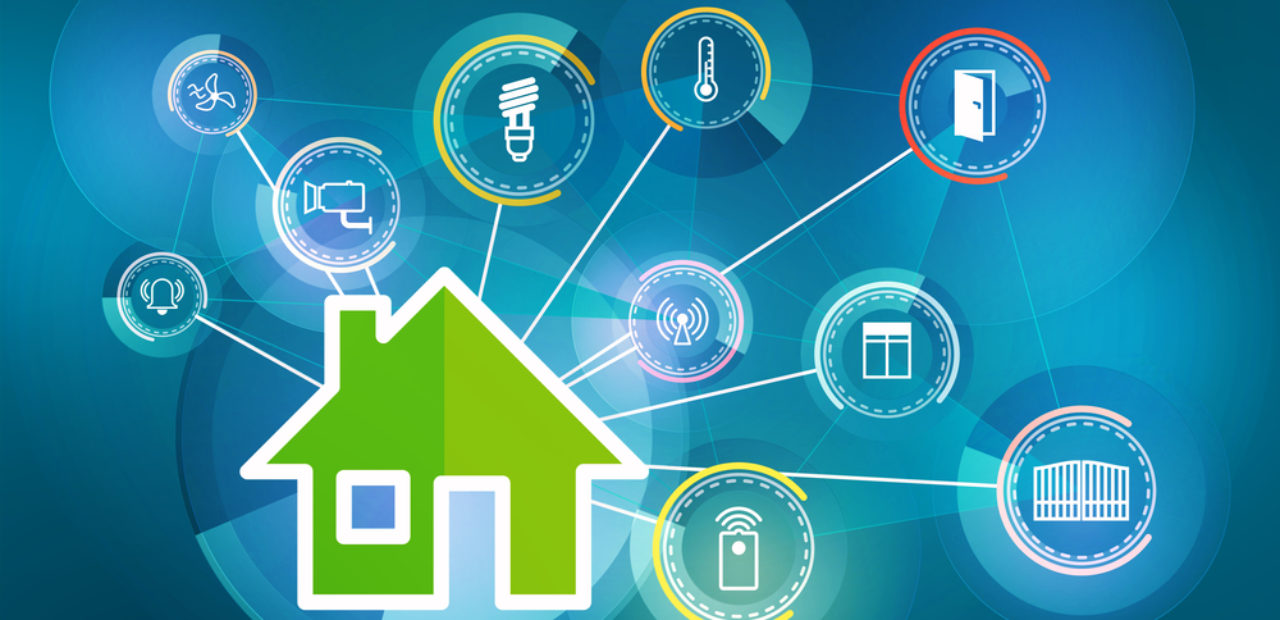
\includegraphics{pics/iot_home.jpg}
  \caption{Interconectarea sistemelor inteligente din clădiri}
  \label{fig:iot_home}
\end{figure}

\subsubsection{Siguranță publică și monitorizarea mediului}
Siguranța publică include menținerea ordinii publice, protecția cetățenilor și protecția de proprietate publică și privată. IoT oferă soluții de monitorizare și urmărire a situațiilor de urgență. Sistemele de urgență ajută la prevenirea și răspunsul în consecință în cazul unui cataclism. Prin colecționarea datelor de la camerele de luat vederi publice sau private se poate ajuta poliția să păstreze liniștea publică. Clădirile care necesită o securitate mai ridicată pot beneficia de sisteme IoT pentru protecție și detecție împotriva intrușilor. Senzori dedicați și camere inteligente,  sistemul GPS\footnote{GPS = Global Positioning System} care oferă date despre poziționare, locație în timp real, precum și utilizarea tehnologiei wireless\footnote{wireless = fără fir} pot ajuta la anticiparea anumitor evenimente.

\subsection{Sănătate}
Internetul lucrurilor va juca un rol important în dezvoltarea de servicii inteligente pentru îmbunătățirea activității sociale a oamenilor. IoT care implică cetățeni și comunități în guvernare și luare de decizii pentru a permite oamenilor să trăiască independent sau să mențină relații sociale și să îmbunătățească sănătatea.

\subsubsection{Diagnosticarea bolilor și tratament}
Industria sănătății va fi puternic influențată de IoT. Senzori inteligenți care permit colectarea de informații vitale de la pacienți(temperatură, tensiune arterială, puls, nivel de colesterol) în timp real  și transmise către un specialist printr-o tehnică de comunicație pentru diagnostic și monitorizare. Rețele BAN\footnote{BAN = Body Area Network} sunt interconectate prin dispozitive purtabile care permit monitorizare de la distanță a pacienților din afara spitalelor. Deasemenea IoT mai poate fi utilizat în identificarea substanțelor, ustensilelor în spitale și inventarierea acestora, astfel pierderea sau furtul acestora fiind mai puțin probabile.

\subsubsection{Stil de viață}
În cadrul acestui subdomeniu, IoT are o largă întrebuințare. Oamenii pot opta să utilizeze dispozitive purtabile care includ senzori de monitorizare a semnelor vitale care pot declanșa alarme medicale în cazul unor probleme de sănătate, precum și ale altor indici de interes pentru utilizator(calorii consumate, distanță parcursă, poziționare). Activitățile zilnice pot fi și acestea urmărite și se pot primi sugestii de schimbare a unor obiceiuri în funcție de scopul setat de utilizator. Pentru persoanele cu handicap vizual sunt dezvoltate aplicații IoT(senzori și aplicații mobile) care le ajută pe acestea să se deplaseze în oraș. 
\begin{figure}[th]
\centering
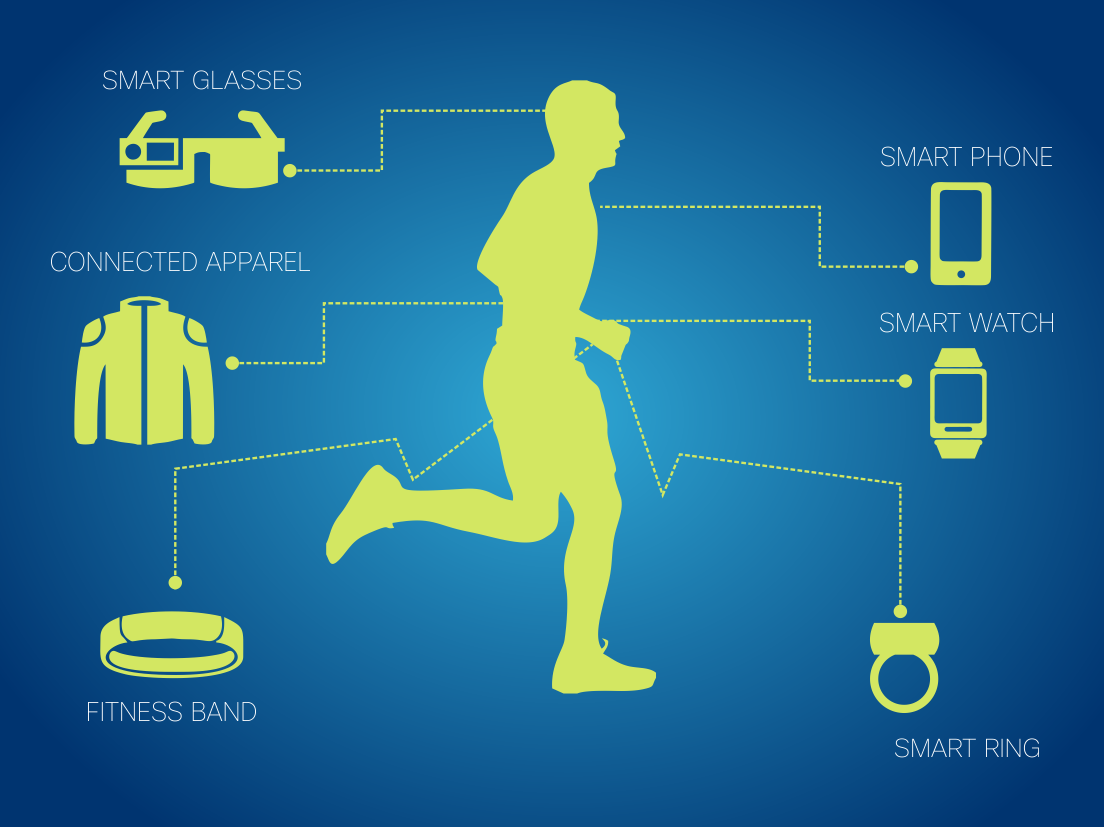
\includegraphics{pics/iot_health.png}
  \caption{Exemplu de sisteme ce ajută la îmbunătățirea stilului de viață}
  \label{fig:iot_health}
\end{figure}

\chapter{Descrierea problemei abordate și a metodei de rezolvare propuse}
În cadrul lucrării se abordează problematica integrării unei noi plăci de dezvoltare în ecosistemul Arduino. \\
Gama SAMR21 de la Atmel cuprinde o serie de microcontrolere cu consum redus ce pot fi utilizate în aplicații care necesită comunicație radio. Kitul de dezvoltare Atmel SAM R21 Xplained Pro este o platformă hardware proiectată de Atmel pentru a se putea evalua microcontrolerul ATSAMR21G18A. \\
Motivele pentru care un dezvoltator de aplicații IoT ar alege o placă de dezvoltare bazată pe microcontrolerul ATSAMR21G18A sunt:
\begin{itemize}
	\item{consumul redus}
	\item{performanța ridicată}
	\item{modulul radio integrat}
\end{itemize}
Când vine vorba de alegerea unui mediu de dezvoltare prietenos cu utilizatorii începători și care suportă o gamă largă de platforme și plăci de dezvoltare, opțiunile sunt limitate, cea mai des aleasă  metodă este utilizarea Arduino IDE. 
Arduino IDE permite utilizatorilor să dezvolte aplicații care folosesc plăci de dezvoltare bazate pe microcontrolere: AVR, SAMD, STM32, Intel ix86, etc. După cum se observă, plăcile de dezvoltare bazate pe microcontrolere SAMR, nu sunt suportate. \\
Tema propusă este să se adauge, la lista de plăci de dezvoltare suportate de către Arduino IDE, și placa Atmel SAMR21 Xplained Pro.

Primul pas în rezolvarea acestei probleme este de a analiza structura proiectului unei alte plăci de dezvoltare și a urma acel model. După analiza proiectului unei plăci de dezvoltare bazate pe SAMD s-a ajuns la concluzia că pentru adăuga o placă de dezvoltare la Arduino IDE trebuie să adăugăm o nouă componentă nucleu care să fie compatibilă cu placa de dezvoltare Atmel SAMR21 Xplained Pro și fișiere de configurare pentru pinii plăcii. 

\chapter{Documentație tehnică}
În capitolul curent se vor prezenta detaliile tehnice folosite în rezolvarea temei propuse.\\
\section{Placa Atmel SAMR21 Xplained Pro}
Pentru a putea duce la bun sfârșit tema propusă, au fost necesare două plăci de dezvoltare bazate pe microcontrolerul ATSAMR21G18A, două plăci Atmel SAM R21 Xplained Pro (Figura ~\ref{fig:samr21}). \\
Placa de dezvoltare Atmel SAM R21 Xplained Pro este o platformă hardware de evaluare a microcontrolerului ATSAMR21G18A, produs de Atmel\cite{samr21ug}. \\
\begin{figure}[th]
\centering
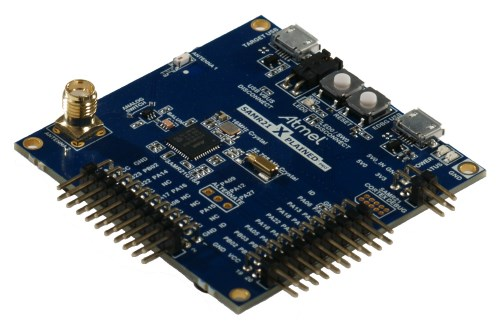
\includegraphics[scale=0.7]{pics/samr21.jpg}
  \caption{Atmel SAMR21 Xplained Pro}
  \label{fig:samr21}
\end{figure}\\
Cele mai importante caracteristici ale plăcii de dezvoltare sunt:
\begin{itemize}
	\item{procesor ARM Cortex-M0+ de până la 48MHz}
	\item{memorie flash 256KB}
	\item{memorie SRAM 32KB}
	\item{mod de consum redus}
	\item{depanator integrat(EDBG)}
		\subitem{interfață USB\footnote{USB = Universal Serial Bus}}
		\subitem{programarea și depanarea prin SWD\footnote{SWD = Serial Wire Debug}}
	\item{pini de intrare și ieșire}
	\item{două butoane mecanice}
	\item{un LED}
	\item{antenă radio}
		\subitem{antenă ceramică\cite{antena}}
		\subitem{un conector SMA\footnote{SMA = SubMiniature version A} pentru antenă externă}
	\item{trei posibilități de alimentare}
		\subitem{extern}
		\subitem{prin depanator USB}
		\subitem{prin USB țintă}
	\item{modulu radio AT86RF233\cite{at86rf}}
	\item{cristal de 32kHz}
	\item{cristal de 16MHz}
\end{itemize}

\subsection{Procesor}
Procesorul ARM Cortex-M0+ are un set de 56 de instrucțiuni, majoritatea pe 16 biți, și operează pe regiștri de 32 de biți fiind proiectat cu scopul de a servi în aplicații cu sisteme integrate\cite{cpu}. Oferă beneficii semnificative dezvoltatorilor, inclusiv:
\begin{itemize}
	\item{arhitectură simplu de învățat și utilizat}
	\item{mod de consum ultra redus}
	\item{procesare de întreruperi de mare performanță}
	\item{compatibil cu procesoare Cortex-M}
	\item{include sistem de protecție a memoriei}
\end{itemize}
Toți regiștrii sunt pe 32 de biți dintre care 13 regiștri sunt de uz general, 3 sunt pentru uz special(SP\footnote{SP = Stack Pointer}, LR\footnote{LR = Link Register}, PC\footnote{PC = Program Counter}). Procesorul ARM Cortex M0+ poate adresa un maxim de 4GB de memorie care sunt împărțiți în memorie pentru cod, SRAM, periferice, RAM extern, dizpozitive externe, magistrala privată a perifericelor și memorie sistem precum în figura ~\ref{fig:memory}.
\begin{figure}[th]
\centering
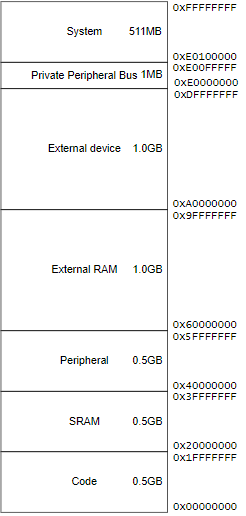
\includegraphics[scale=0.7]{pics/memory_map.png}
  \caption{Modelul structurării memoriei\cite{memmap}}
  \label{fig:memory}
\end{figure} \\
Procesorul Cortex-M0+ este construit pe un nucleu optimizat pentru consum și dimensiune, cu un pipeline pe două niveluri(Figura ~\ref{fig:pipeline}) și o arhitectură von Neumann.
\begin{figure}[bh]
\centering
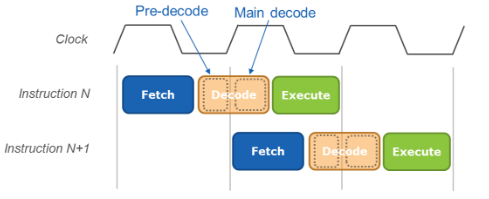
\includegraphics[scale=0.7]{pics/pipeline.png}
  \caption{Pipeline pe două niveluri\cite{pipeline}}
  \label{fig:pipeline}
\end{figure} \\
Acest procesor implementează arhitectura ARMv6-M, care e bazată pe un set de instrucțiuni de 16 biți Thumb și include tehnologie Thumb-2. Acest lucru oferă performanțele excepționale așteptate de la un procesor cu arhitectură pe 32 de biți, cu o densitate mai mare a codului decât microcontrolerele de 8 sau 16 biți.

Procesorul ARM Cortex M0+ dispune de un controler pentru întreruperi, NVIC\footnote{NVIC = Nested Vectored Interrupt Controller}, care se ocupă cu gestionarea acestora. NVIC permite prioritizarea întreruperilor, mascarea aceastora și definirea de rutine care se apelează la declanșarea unei întreruperi. Executarea rutinelor se face dupa 15 sau 16 cicli de ceas, în acest timp, procesorul gestionează trecerea de la stiva funcției executate la momentul de timp actul la stiva pentru rutina de întrerupere.

\subsection{Depanatorul integrat}
Placa Atmel SAM R21 Xplained Pro conține depanatorul Atmel EDBG\footnote{EDBG = Atmel Embedded Debugger} pentru depanarea codului sursă direct pe placa de dezvoltare. EDBG este compus din trei interfețe: un depanator, un port de comunicație serială COM\footnote{COM = Communication Port} și o interfață de date DGI\footnote{DGI = Data Gateway Interface}.\\
Depanatorul este utilizat pentru depanarea codului prin rularea lui pe placa de dezvoltare și verificarea bunei funcționări.\\
Portul de comunicație serială este conectat la o interfață UART\footnote{UART = Universal Asynchronous receiver-transmitter}, interfață de comunicație serială asincronă, și oferă posibilitatea de comunicare cu microcontrolerul prin terminal software. Oferă viteză de transfer ridicată, opțiuni de paritate a datelor transmise și de bit de stop.\\
Interfața de date e compusă din mai multe interfețe de comunicație cu computerul gazdă. Comunicația pe aceste interfețe este bidirecțională și poate fi folosită pentru notificarea în legătură cu declanșarea unor evenimente sau pur și simplu pentru transmisie de date.

\subsection{Surse de alimentare}
Placa de dezvoltare Atmel SAM R21 Xplained Pro poate fi alimentată în mai multe moduri, după cum arată tabela ~\ref{tab:surse}. \\
Placa de dezvoltare va detecta automat ce surse de alimentare sunt disponibile și va alege dintre acestea în funcție de următoarele priorități:
\begin{enumerate}
	\item{Extern}
	\item{Prin depanator USB}
	\item{Prin USB țintă}
\end{enumerate}

\begin{table}[th]\small\linespread{1}
\caption{Surse alimentare}
\label{tab:surse}
\begin{tabular}{l >{\raggedright\arraybackslash}p{8cm} >{\raggedright\arraybackslash}p{4cm}}
\textbf{Intrare} & \textbf{Tensiune} & \textbf{Curent} \\\hline
\textbf{Extern} & 5V \SI{\pm 100}mV pentru utilizare ca gazdă.  De la 4.3V până la 5.5V dacă nu e necesară utilizarea ca gazdă & Minimul recomandat e 1A pentru a putea să susțină toate dispozitivele conectate. Recomandat este maxim 2A.\\\hline
\textbf{Prin depanator USB} & De la 4.4V până la 5.25V & 500mA \\
\hline
\textbf{\textit{Prin USB țintă}} & De la 4.4V până la 5.25V & 500mA \\
\hline
\end{tabular}
\end{table}

\subsection{Periferice}
\subsubsection{Butoane mecanice}
Placa de dezvoltare conține doua butoane mecanice. Un buton este butonul de reset care este conectat ma linia de reset a microcontrolerului, iar celălalt buton este un buton de uz general care poate fi configurat. Când unul dintre butoane este apăsat, va lega linia la GND\footnote{GND = ground (masă)}.

\subsubsection{LED}
Există un LED, numit LED0, disponibil pe placa de dezvoltare Atmel SAM R21 Xplained Pro care poate fi activat sau dezactivat. Pentru a activa ledul, este necesar să legăm linia la GND.

\subsubsection{Radio}
Principalul scop al plăcii de dezvoltare Atmel SAMR21 Xplained Pro, este să pună în evidență capacitățile de comunicație radio ale microcontrolerului ATSAMR21G18A. Modulul AT86RF233, este un transmițător radio de consum redus proiectat pentru uz industrial și pentru aplicații ce folosesc protocoalele IEEE 802.15.4, Zigbee, SP100, WirelessHART, ISM. Este un periferic SPI-to-antenna, adică folosește o comunicație SPI pentru a permite interacțiunea dintre microcontroler și antenă. Modulul este compus dintr-un transmițător radio analogic și un demodulator digital care include sincronizare pe domeniile timp și frecvență. Toate componentele necesare sunt integrate într-un singur chip, astfel minimizând numărul de componente externe: antena, cristal de quartz și capacități de decuplare.

Această placă dispune de posibilitatea de a alege dintre două antene, antena ceramică sau antena conectată la conectorul SMA. Această posibilitate o oferă intrerupătorul AS222-92LF\cite{switch} conectat la doi pini de la microcontroler, RFCTRL1 și RFCTRL2, prin care microcontrolerul alege care antenă va fi utilizată în procesul de comunicație. Alegerea se face pe baza ieșirii unui transformator 2450BM15A0015\cite{balun} care este conectat la 2 pini diferențiali de antenă de la microcontroler ca în figura ~\ref{fig:antena}. \\

\begin{figure}[!htb]
\centering
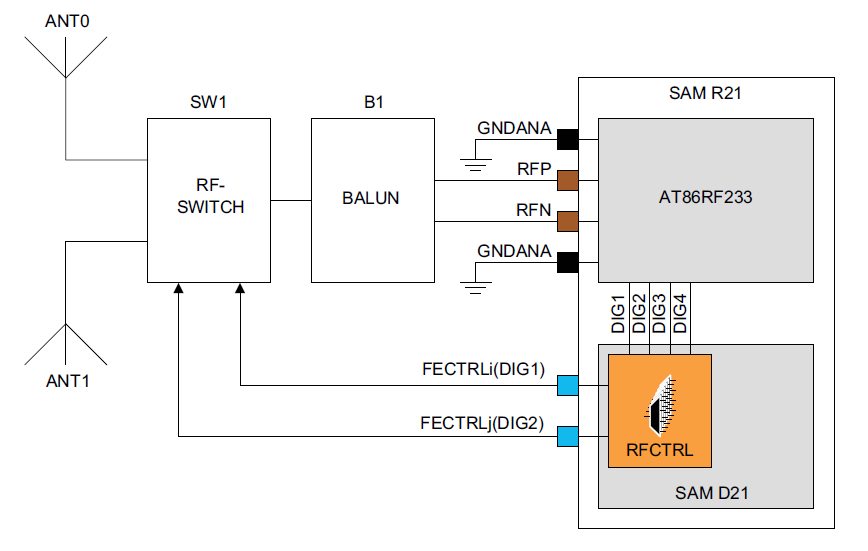
\includegraphics[scale=0.5]{pics/antena.png}
  \caption{Schema de legare a antenei}
  \label{fig:antena}
\end{figure}


\section{Arduino IDE}
Înainte de a trece mai departe, este necesară prezentarea structurii unui proiect din Arduino IDE și detalii despre cum se ajunge la obiectul final încărcat pe placa de dezvoltare țintă.
Un proiect în Arduino IDE este împărțit în 4 părți cu cod sursă:
\begin{itemize}
	\item{core\footnote{core = nucleu} - aici este codul de bază pentru fiecare platformă}
	\item{variant\footnote{variant = se referă la placa de dezvoltare} - aici se află fișiere de configurare pentru placa de dezvoltare}
	\item{sketch\footnote{sketch = schiță} - aici se află codul utilizatorului}
	\item{library\footnote{library = bibliotecă} - aici se află codul sursă pentru bibliotecile opționale}
\end{itemize}
Punctul de intrare în proiect este fișierul \textit{main.c} în funcția \textit{main}, din \textit{core}, în care se apelează funcțiile scrise de utilizator în fișierul cu extensia \textit{.ino}, \textit{setup și loop}, din \textit{sketch}. \\
Procesul de build\footnote{build = construire} al proiecului constă în compilarea tuturor fișierelor sursă, cu fișierele header corespunzătoare, din toate cele 4 părți ale proiectului și asamblarea lor într-un singur fișier rezultat cu extensia \textit{.hex}, stocat la o locație temporară. Fișierul rezultat este mai apoi urcat în memoria microcontrolerului țintă și executat.

\subsection{Dezvoltare proiect}
Pentru a implementa tema propusă, se vor creea 3 din cele 4 părți componente ale unui proietct în Arduino IDE. În final, cele 3 părți formează pachetul care va fi arhivat și stocat online, iar oricine va dori să utilizeze o placă de dezvoltare de acest tip, va putea folosi acest pachet. La baza acestui pachet se află câteva fișiere de configurare a programatoarelor folosite de această placă de dezvoltare, de configurare a plăcii de dezvoltare și de configurare a procesului de build.

Fișierul \textit{boards.txt} conține informații esențiale cu privire la placa de dezvoltare cum ar fi:
\begin{itemize}
	\item{name - numele plăcii de dezvoltare}
	\item{vid - număr de identificare a vânzătorului}
	\item{pid - număr de identificare a producătorului}
	\item{upload tool - unealta folosită pentru a urca codul pe placa de dezvoltare precum și parametri de configurare a acesteia} 
	\item{mcu - procesorul pentru care se face build}
	\item{core - nucleul utilizat}
	\item{ldscript - linker script}
	\item{variant - variantul folosit}
\end{itemize}
Fișierul folosit în cadrul proiectului conține toate acele informații, dar și alte informații suplimentare necesare funcționării corecte a programării plăcii de dezvoltare(Figura ~\ref{fig:boards}).
\begin{figure}[h]
\centering
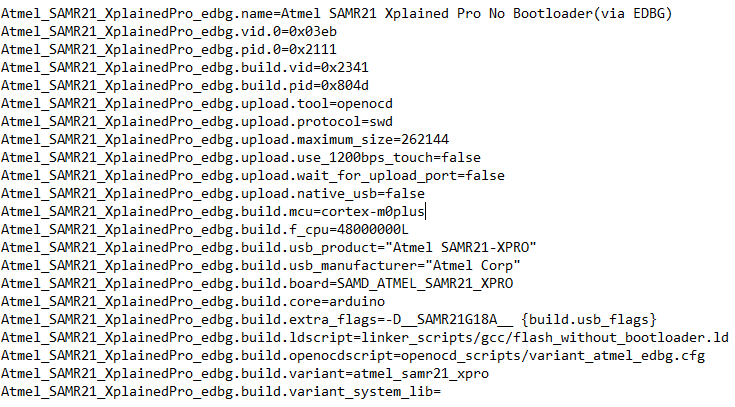
\includegraphics[scale=0.7]{pics/boards.png}
  \caption{Fișierul \textit{boards.txt} asociat pachetului}
  \label{fig:boards}
\end{figure}\\
Pentru configurarea programatorului folosit este nevoie de un fișier în care se specifică numele programatorului, care se va găsi în meniul cu programatoare din Arduino IDE, și tipul de comunicație folosit , în cazul proiectului de față fiind USB. Mai este necesar un fișier numit \textit{platform.txt} în care se specifică argumente pasate compilatorului, linkerului sau asamblorului.

\subsubsection{Core}
Ținând cont de faptul că placa de dezvoltare Atmel SAM R21 Xplained Pro este un dispozitiv SAM R21,  care este compus din SAM D21 și modulul radio AT86RF233, codul sursă pentru core va fi asemănător cu cel pentru SAM D21, cu modificările aferente. \\
După o examinare amănunțită a documentației microcontrolerului SAM D21G în comparație cu cea a microcontrolerului SAM R21G, se observă câteva diferențe majore:
\begin{itemize}
	\item{numărul de module TC\footnote{TC = Timer Counter} a scăzut de la 5 la 3}
	\item{pentru SAM R21G nu avem modul DAC\footnote{DAC = Digital to Analog Converter}}
	\item{pentru SAM R21G nu avem modul I2S\footnote{I2S = Inter-IC Sound Interface}}
\end{itemize}
Pentru a ne putea folosi de codul deja scris pentru plăcile de dezvoltare bazate pe SAM D21, este necesară modificarea acestuia în conformitate cu documentația oferită de producător pentru SAM R21G. Configurarea corectă a acestuia implică modificarea numărului de module TC și eliminarea inițializării modulului DAC, pe care microcontrolerele SAM D21 le au.
Fiecare întrerupere are asociată o rutină care se execută când este declanșată acea întrerupere. Aceste rutine sunt setate în în mod implicit în codul de Arduino să apeleze funcție numită \textit{Dummy\_Handler} care va bloca programul în cazul unei întreruperi nedorite de utilizator. La setarea unei întreruperi prin apelul la functia \textit{attachInterrupt}, se modifică vectorul de întreruperi, variabila \textit{exception\_table}(Figura ~\ref{fig:interrupts}), în care sunt stocate adresele rutinelor de întrerupere pentru fiecare dintre întreruperi. 
\begin{figure}[h]
\centering
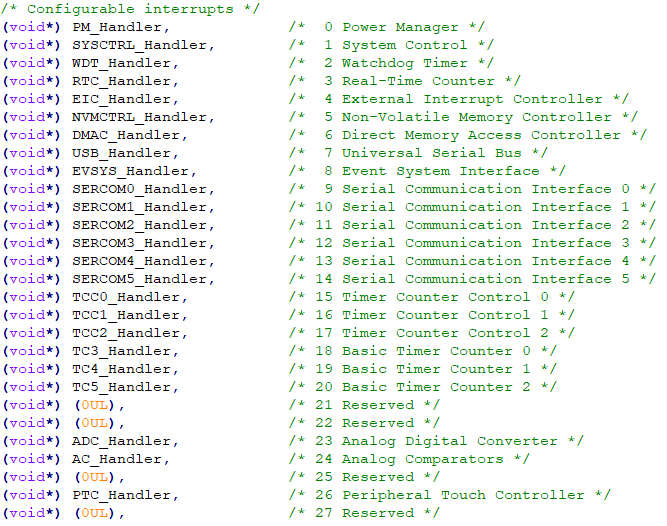
\includegraphics[scale=0.6]{pics/interrupt_vector.png}
  \caption{Întreruperile configurabile din \textit{exception\_table}}
  \label{fig:interrupts}
\end{figure}\\
Această variabilă, este pusă implicit în secțiunea de cod numită \textit{.isr\_vector} folosind \textbf{\_\_attribute\_\_ ((section()))}. Astfel, în fișierul binar rezultat, această variabilă va fi pusă în memorie unde indică scriptul pentru linker. Pentru a configura corect întreruperile pentru placa de dezvoltare Atmel SAM R21 Xplained Pro, trebuie să scoatem definirea rutinelor pentru modulele DAC, I2S și TC. Astvel, se vor înlătura \textit{TC6\_Handler, TC7\_Handler, DAC\_Handler, I2S\_Handler}.

La declanșarea întreruperii de reset, fie prin apăsarea butonului sau software, se inițializează datele din RAM cu valorile aflate în zona flash, zona de date neinițializate se setează cu 0, iar apoi se apelează funcția de inițializare a modulelor care activează ceasul pentru toate modulele, pornește modulele esențiale. După ce inițializarea s-a terminat cu succes, se apelează funcția main, care va apela mai departe codul din sketch, al utilizatorului.

Este necesară și îndepărtarea codului de inițializare a modulului DAC, deoarece pentru microcontrolerul SAM D21G se pornea ceas și pentru modulul de DAC, iar la microcontrolerul SAM R21G nu există, setarea acelui bit poate duce la un comportament nedefinit. În final, este necesară doar activarea modulului ADC în PM\footnote{PM = Power Manager} setând bitul ADC din registrul APBCMASK(Figura ~\ref{fig:apbcmask}).
\begin{figure}[h]
\centering
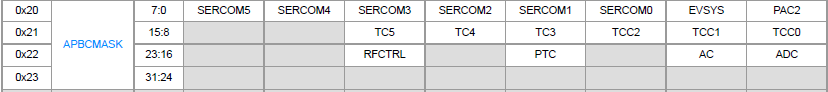
\includegraphics[scale=0.7]{pics/apbcmask.png}
  \caption{Formatul registrului APBCMASK}
  \label{fig:apbcmask}
\end{figure}\\
În fișierul \textit{WVariant.h}, în enumul \textit{EPioType}, mai definim un element numit \textit{PIO\_RADIO} care va avea valoarea 5. Această modificare va ajuta ulterior la definirea pinilor radio pentru placa de dezvoltare, care au nevoie de funcția F(Figura ~\ref{fig:alternatefunctions}).
\begin{figure}[h]
\centering
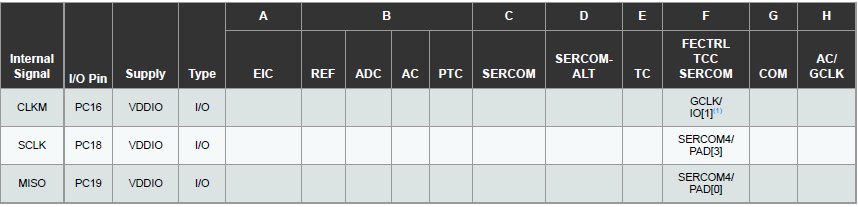
\includegraphics[scale=0.7]{pics/alternate_functions.png}
  \caption{Funcțiile alternative ale pinilor radio}
  \label{fig:alternatefunctions}
\end{figure}\\

\subsubsection{Variant}
În această parte a proiectului sunt definite configurațiile pinilor plăcii de dezvoltare, precum și diferite scripturi pentru linker.
 În fișierul \textit{variant.cpp}, pinii GPIO\footnote{GPIO = General Purpose I/O} sunt descriși printr-o structură numită \textit{PinDescription}(Figura ~\ref{fig:pindescription}).
\begin{figure}[h]
\centering
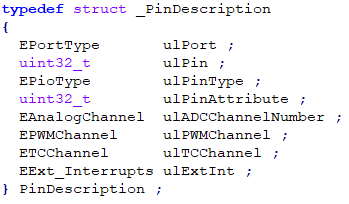
\includegraphics[scale=0.9]{pics/pindescription.png}
  \caption{Structura folosită pentru definirea pinilor GPIO}
  \label{fig:pindescription}
\end{figure}\\
\textit{EPortType} reprezintă portul de care aparține pinul respectiv, acesta putând fi: PORTA, PORTB, PORTC, iar următorul membru al structurii conține numărul pinului. Membrul \textit{ulPinType} conține informații despre funcția periferică alternativă pe care o îndeplinește pinul, iar următoarele câmpuri sunt utilizate pentru setarea de atribute, intreruperi, canal pentru ADC.\\
Fișierul conține un vector de structuri de acest tip care reprezintă pinii pe care îi poate folosi un utilizator când lucrează cu această placă de dezvoltare. Fișierul header mai conține și niște definiții pentru anumiți pini care vor fi utilizați ulterior în cod, spre exemplu pinii pentru modulul radio.

Scripturile pentru linker reprezintă un set de reguli pe care linkerul le urmează când procesul de build ajunge în faza de linkare. Aceste reguli se referă la locul unde sunt stocate variabilele, codul și simbolurile globale. Acest script pentru linker este format din două părți:
\begin{itemize}
\item{Memory - în care se declară memoriile disponibile, adresele de început și dimensiunile acestora}
\item{Sections - în care se atribuie fiecare secțiune de memorie din obiectele compilate la una din memoriile disponibile}
\end{itemize}
Un exemplu de secvență în care se definesc memoriile disponibile se poate observa în Figura ~\ref{fig:scriptmemory}, unde sunt definite două memorii, FLASH și RAM fiecare cu dimensiunile respective.
\begin{figure}[h]
\centering
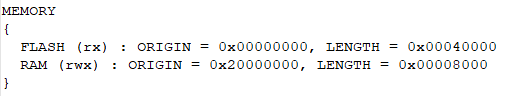
\includegraphics[scale=0.9]{pics/scriptmemory.png}
  \caption{Memoriile definite în scriptul pentru linker}
  \label{fig:scriptmemory}
\end{figure}\\
În segmentul \textit{Sections} se pot rula diferite comenzi, însă cele mai utilizate în cadrul acestui proiect sunt acelea de a selecta secțiuni, de a le atribui la una din memoriile definite și de a defini simboluri care pot fi folosite în cod pe parcursul dezvoltării. Un exemplu este zona de date \textit{.bss}(Figura ~\ref{fig:bssscript}) care conține toate variabilele globale neinițializate încadrate între două simboluri globale \textit{\_\_bss\_start\_\_, \_\_bss\_end\_\_} folosite în general la determinarea dimensiunii.
\begin{figure}[h]
\centering
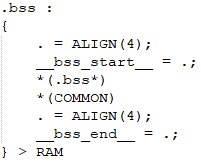
\includegraphics[scale=0.9]{pics/bss.png}
  \caption{Zona de memorie .bss din scriptul pentru linker}
  \label{fig:bssscript}
\end{figure}\\

\subsubsection{Library}
Codul sursă pentru funcționalitatea radio se află în această parte a proiectului. Implementarea pentru biblioteca radio care oferă funcționalitatea dorită folosind modului AT86RF233 există în sistemul de operare în timp real destinat aplicațiiolor IoT, RIOT-OS. Translatarea acestui cod la o bibliotecă scrisă în C++ pentru Arduino va fi folosită în realizarea proiectului\cite{msolters}.

Pentru a putea utiliza modulul radio AT86RF233 este necesară configurarea corectă a acestuia. Motivul pentru care configurarea a fost implementată aici și nu în inițializarea plăcii de dezvoltare este că activarea acestui modul radio duce la un consum adițional care va exista doar când este folosită această bibliotecă.
În fișierul sursă al clasei \textit{AT86RF2xx} am adăugat niște metode adiționale care vor ajuta la configurarea corectă a microcontrolerului pentru a comunica cu modulul radio prin intermediul unei interfețe SPI\footnote{SPI = Serial Peripheral Interface}(Figura ~\ref{fig:spi}). 
\begin{figure}[h]
\centering
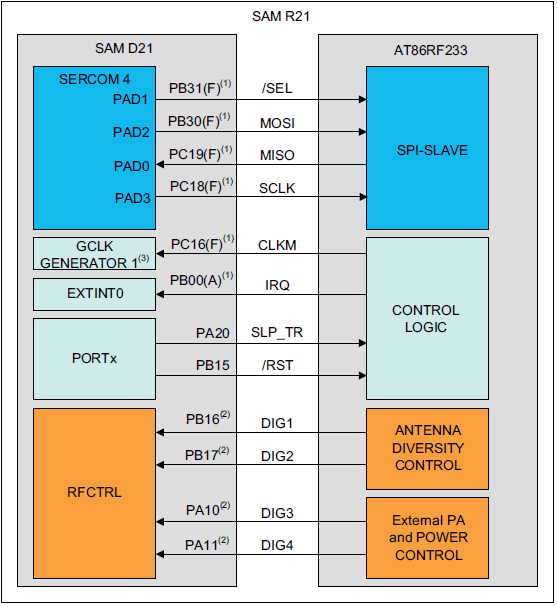
\includegraphics[scale=0.9]{pics/spi.png}
  \caption{Interfața de comunicație dintre microcontreler și modulul radio\cite{samr21ug}}
  \label{fig:spi}
\end{figure}\\
Etapele configurării sunt:
\begin{enumerate}
	\item{Setare pin /SEL ca ieșire și setarea ieșirii acestuia pe High}
	\item{Activare Sercom4}
	\item{Setarea ceasului corect și pornirea acestuia pentru Sercom4\footnote{Sercom = Serial Communication Interface}}
	\item{Setare pini MISO, MOSI, SCK ca intrare cu pulldown}
	\item{Pornire comunicație SPI folosind biblioteca SPI din Arduino}
	\item{Configurare întrerupere}
\end{enumerate}

Pentru setarea pinilor ne folosim de faptul că am configurat corect intrările din \textit{variant} și putem astfel să apelăm rutinele din Arduino și să fim siguri că se întâmplă ceea ce dorim. La apelul funcției \textit{pinMode} se setează în registrul DIR din PORT direcția dorită(High sau Low). Pentru a putea folosi pinii pe comunicația SPI cu modulul radio, intern biblioteca SPI setează niște funcții periferice alternative, și anume funcția F, în registrul PMUX din PORT și activează multiplexorul din registrul PINCFG folosindu-se de registrul WRCONFIG, care ajută la configurarea unui grup de pini(Figura ~\ref{fig:pinperipheral}).
\begin{figure}[h]
\centering
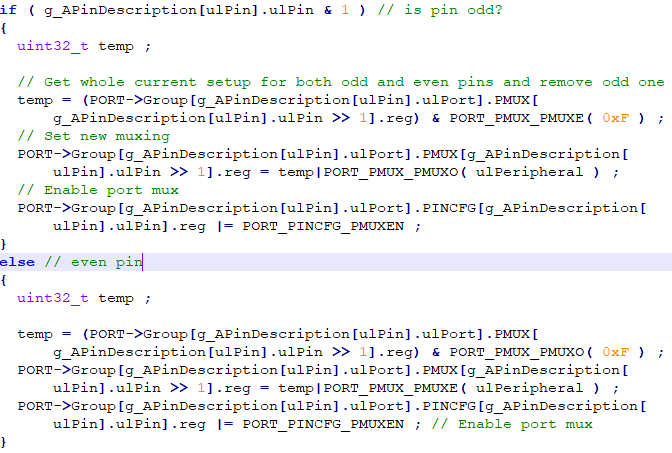
\includegraphics[scale=0.8]{pics/pinperipheral.png}
  \caption{Pașii urmați pentru setarea funcției periferice}
  \label{fig:pinperipheral}
\end{figure}\\
Deoarece registrii PMUX[0-15], în care sunt stocate funcțiile periferice alternative pentru pini sunt împărțiți în două părți egale, una pentru pinul cu număr par, iar cealaltă pentru pinul cu număr impar, este necesară acea verificare pentru a ști să prezervăm setările deja făcute pentru pinul care folosește același registru, dar de paritate diferită.\\
Pentru activarea Sercom4 se setează bitul corespunzător din registrul APBCMASK din PM. Configurarea ceasului pentru Sercom4 se face folosing regiștrii din GCLK\footnote{GCLK = Generic Clock Controller}. Astfel, primul pas este să se dezactiveze canalul de ceas pentru Sercom4\_core, urmată de selectarea ceasului dorit prin scrierea în registrul CLKCTRL din GCLK a numărului de identificare corespunzător și a sursei de ceas dorite(în cazul nostru 0, ceasul principal), iar apoi activarea ceasului. Aceiași pași se urmează și la activarea Sercom4\_slow. Sercom4\_core este necesar când operează ca master, iar Sercom4\_slow este necesar pentru diferite funcții.
Pentru setarea întreruperii este necesară structura pinului corespunzător să fie configurată corect, iar rutinele din Arduino vor seta corect și întreruperea pentru modulul radio. Pinul pentru întreruperea venită de la modulul radio, IRQ, va fi setat ca pin de intrare cu pull down iar pentru atașarea unei rutine de întrerupere se va apela funcția \textit{attachInterrupt}, care va seta pe întreruperea externă 0, EXTINT0, o întrerupere pe ciclul crescător al semnalului.

După ce configurarea s-a terminat, biblioteca radio verifică dacă poate citi cu succes registrul \textit{PART\_NUM} din modulul radio, folosind comunicația SPI. \\
Pentru a comunica cu modulul radio prin intemediul SPI s-au definit mai multe moduri de acces:
\begin{itemize}
	\item Register access citire și scriere
	\item Frame Buffer access citire și scriere
	\item SRAM access citire și scriere
\end{itemize}
Pentru a putea selecta unul dintre cele 6 moduri disponibile pentru comunicația cu modulul AT86RF233, se transmite un octet care va coda comanda după cum arată Figura ~\ref{fig:commandbyte}.
\begin{figure}[h]
\centering
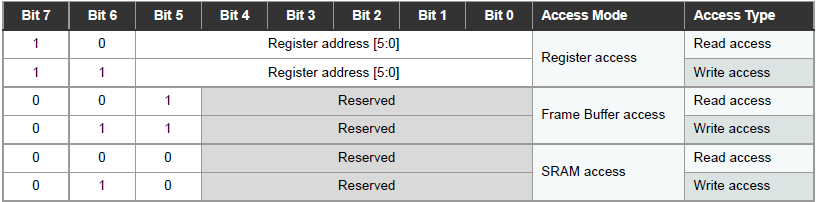
\includegraphics[scale=0.8]{pics/commandbyte.png}
  \caption{Descrierea comenzilor transmise pe SPI\cite{samr21ds}}
  \label{fig:commandbyte}
\end{figure}\\
Modul \textit{Register Access} este folosit pentru a scrie sau a citi regiștri modulului AT86RF233, adresele acestora se află în intervalul 0x00-0x3F. Acest mod de acces reprezintă o transmisie de doi octeți, operație declanșată de setarea bitului de selecție /SEL pe LOW. Primul octet este format din doi biți care reprezintă comanda transmisă(citire sau scriere), urmată de 6 biți în care se stochează adresa registrului accesat, iar cel de al doilea octet reprezintă valoarea care se dorește a fi scrisă în acel registru în cazul operației de scriere, în cazul operației de citire nu contează. 
Protocolul SPI este un protocol de transmisie dublă, adică în timpul tranferului de date de la microcontroler la modulul radio se face și un transfer invers care în cazul citirii este valoarea cerută, iar în cazul operației de scriere este o valoare care reflectă starea modulului radio.\\
În biblioteca radio implementată, acest mod de acces este utilizat pentru citira stărilor modulului radio și pentru începerea transmisiei de date. Cel mai des utilizați regiștri sunt: TRX\_STATE, TRX\_CTRL\_0, TRX\_CTRL\_2 și IRQ\_MASK\cite{samr21ds}.

\textit{Frame Buffer} este o zonă de memorie SRAM de 128 de octeți cu două porturi. Un port este conectat la interfața SPI, celălalt la transmițătorul și receptorul intern. Ambele porturi sunt independente și accesibile simultan. Acest buffer utilizează spațiul de adrese SRAM, 0x00-0x7F, pentru operații de transmisie și recepție și poate stoca un singur cadru IEEE 802.15.4 de lungime maximă la același moment de timp. Un cadru IEEE 802.15.4 este format din două părți, o secțiune de preambul generată intern și partea din \textit{Frame buffer}, accesibilă utilizatorului. În partea de \textit{Frame buffer} se rețin și date despre lungimea cadrului, puterea sau calitatea acestuia(LQI\footnote{LQI = Link Quality Indication}), o estimare a puterii semnalului primit(ED\footnote{ED = Energy Detection}), etc(Figura~\ref{fig:frame}).
\begin{figure}[h]
\centering
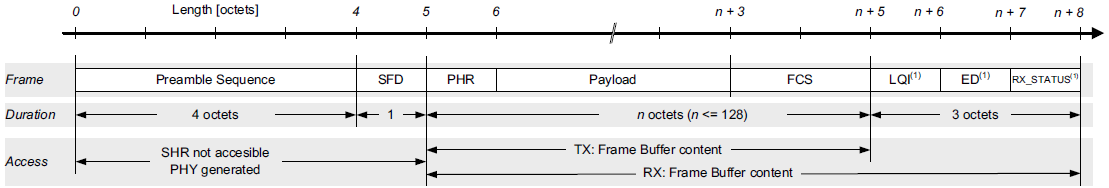
\includegraphics[scale=0.6]{pics/frame.png}
  \caption{Formatul unui cadru IEEE 802.15.4\cite{samr21ds}}
  \label{fig:frame}
\end{figure}\\
Modul de acces \textit{Frame buffer} este utilizat când se dorește citirea sau scrierea unui cadru IEEE 802.15.4. Adresa de scriere sau citire este întotdeauna resetată la 0 și incrementată, astfel pentru a putea citi sau scrie informațiiile adiționale despre cadre.

Spre deosebire de modul de acces \textit{Frame buffer}, modul de acces SRAM, este utilizat pentru a scrie în bufferul pentru cadru începând de la o adresă specificată. Oferă posibilitatea accesului direct la datele utile de la adresa dorită fără să se mai urmeze procesul de incrementare pe care îl abordează accesul \textit{Frame Buffer}.\\
În biblioteca radio, modul de acces \textit{Frame Buffer} este folosit doar pentru citirea dimensiunii unui cadru primit, iar în rest, pentru transmisia cadrului se folosește modul de acces SRAM. Astfel, pentru transmiterea unui șir de octeți se apelează următoarele metode din cadrul clasei AT86RF2XX:
\begin{itemize}
\item tx\_prepare
\item tx\_load
\item tx\_exec
\end{itemize}
În cadrul funcției \textit{tx\_prepare} se verifică starea modulului,  dacă este ocupat se așteaptă eliberarea acestuia, iar dacă primește un cadru se anulează transmisia. Se contunuă cu setarea stării de așteptare transmitere.
Funcția de \textit{tx\_load} are ca parametri șirul de octeți care vor fi transmiși, lungimea șirului și indicele de unde va începe scrierea. Datorită faptului că valoarea câmpului PHR este de un octet, indicele de unde va începe scrierea va fi egal cu 1. Pentru a scrie în memoria SRAM se apelează funcția de transfer din clasa SPI care va pune în registrul de date octetul care se dorește a fi transmis spre modulul radio. Astfel, datele transmise sunt, comanda care selectează modul de acces, indicele de la care se începe scrierea și un număr de octeți egal cu lungimea șirului transmis.
Pentru a porni transmisia, în metoda \textit{tx\_exec}, se scrie dimensiunea cadrului IEEE 802.15.4 care va urma a fi transmis, aceasta va fi egală cu dimensiunea șirului de octeți la care se mai adaugă un octet pentru dimensiunea cadrului, și se va scrie în registrul de stare, comanda de pornire a transmisiei. Toată această procedură poate fi observată în Figura~\ref{fig:send}.
\begin{figure}[h]
\centering
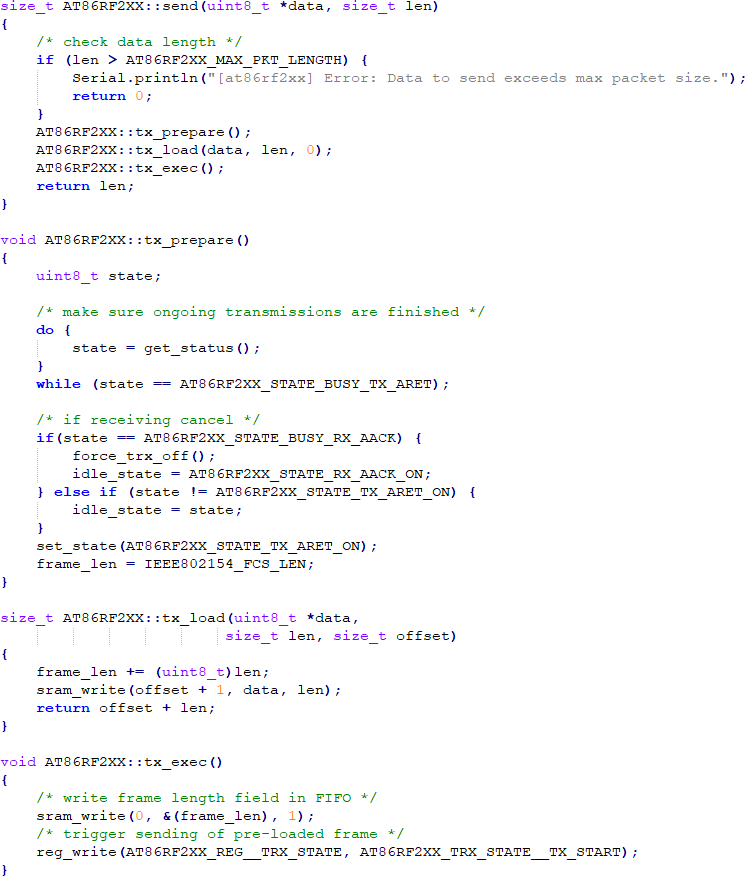
\includegraphics[scale=0.68]{pics/send.png}
  \caption{Implementarea transmisieu unui șir de octeți}
  \label{fig:send}
\end{figure}\\

\subsection{Adăugare proiect}
Pentru adăugarea unei noi plăci de dezvoltare la mediul de dezvoltare Arduino IDE, este necesară crearea unui fișier de tip json\footnote{JSON = JavaScript Object Notation} în care se scriu configurațiile pentru pachetul corespunzător plăcii de dezvoltare.
Fișierul json trebuie să conțină următoarele câmpuri:
\begin{itemize}
	\item{name - numele pe care îl va avea pachetul}
	\item{maintainer - numele celui care menține codul}
	\item{websiteURL - un url către un site web al companiei}
	\item{help}
	\item{platforms}
		\subitem{name - numele plăcii de dezvoltare}
		\subitem{arhitecturre - arhitectura pe care se bazează placa de dezvoltare}
		\subitem{version - versiunea pachetului}
		\subitem{category - de obicei este Contributed, doar cei de la Arduino pot schimba}
		\subitem{url - link către o arhivă cu codul sursă}
		\subitem{archiveFilename - numele arhivei}
		\subitem{checksum - pentru verificare se cere un mesaj de autentificare}
		\subitem{size - mărimea arhivei}
		\subitem{boards}
		\subitem{toolsDependencies - secțiunea cu dependențele de alte utilitare}
	\item{tools - aici se specifică explicit de unde se pot luat utilitarele}
\end{itemize}
Un exemplu de fișier de configurare se poate vedea în figura ~\ref{fig:json}.
\begin{figure}[!htb]
\centering
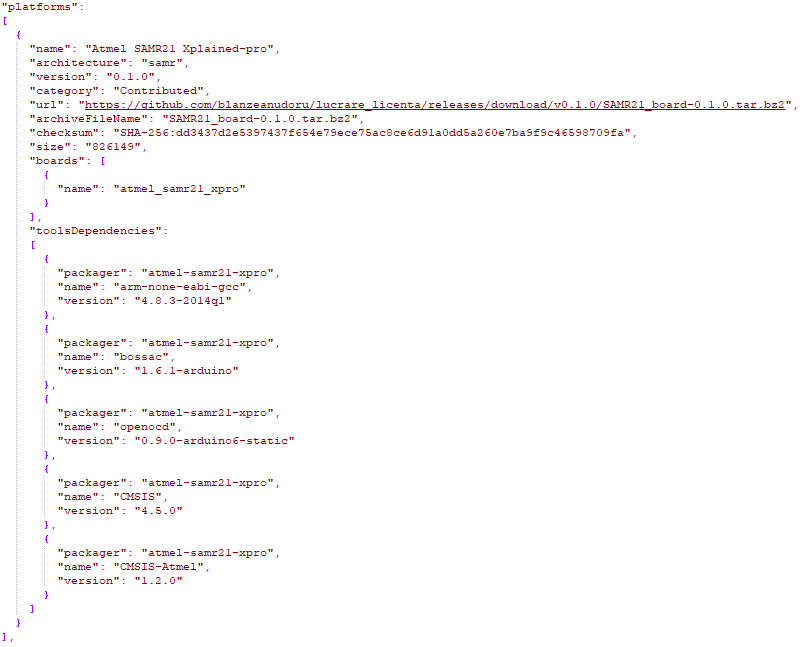
\includegraphics[scale=0.8]{pics/json.png}
  \caption{Exemplu de fișier de configurare}
  \label{fig:json}
\end{figure}

\section{Rezultate obținute}

\chapter{Concluzii și dezvoltări ulterioare}


%BIBLIOGRAFIE
\begin{thebibliography}{9}
\bibitem{theiot}
Keyur K Patel, Sunil M Patel. 
\textit{Internet of Things-IOT: Definition, Characteristics, Architecture, Enabling Technologies, Application \& Future Challenges}.
ISSN 2321 3361, 2016 IJESC\\
\href{http://ijesc.org/upload/8e9af2eca2e1119b895544fd60c3b857.Internet\%20of\%20Things-IOT\%20Definition,\%20Characteristics,\%20Architecture,\%20Enabling\%20Technologies,\%20Application\%20\&\%20Future\%20Challenges.pdf}{http://ijesc.org/upload/8e9af2eca2e1119b895544fd60c3b857.Internet\%20of\%20Things-IOT\%20Definition,\%20Characteristics,\%20Architecture,\%20Enabling\%20Technologies,\%20Application\%20\&\%20Future\%20Challenges.pdf} accesat la data 10/06/2018.

\bibitem{study}
Padraig Scully.
\textit{The Top 10 IoT Segments in 2018 – based on 1,600 real IoT projects}. 
2018 ranking of Top IoT Segments\\
\href{https://iot-analytics.com/top-10-iot-segments-2018-real-iot-projects/}{https://iot-analytics.com/top-10-iot-segments-2018-real-iot-projects/} accesat la data 10/06/2018.

\bibitem{iotfields}
Ran Liu, Jinfeng Wang.
\textit{Internet of Things: Application and Prospect }
MATEC Web of Conferences 100, 02034 (2017)\\
\href{https://www.matec-conferences.org/articles/matecconf/pdf/2017/14/matecconf\_gcmm2017\_02034.pdf}{https://www.matec-conferences.org/articles/matecconf/pdf/2017/14/matecconf\_gcmm2017\_02034.pdf} accesat la data 10/06/2018.


\bibitem{lowpowerimportance}
Sayfe Kiaei, Eby G. Friedman.
\textit{Introduction to the Special Issue on Low Power Wireless Communications}.
IEEE TRANSACTIONS ON CIRCUITS AND SYSTEMS—II: ANALOG AND DIGITAL SIGNAL PROCESSING, VOL. 44, NO. 6, JUNE 1997.\\
\href{https://ieeexplore.ieee.org/stamp/stamp.jsp?arnumber=868450}{https://ieeexplore.ieee.org/stamp/stamp.jsp?arnumber=868450} accesat la data 10/06/2018.

\bibitem{lowpowervsperformance}
JeongGil Ko, Kevin Klues, Christian Richter, Wanja Hofer, Branislav Kusy, Michael Bruenig, Thomas Schmid, Qiang Wang, Prabal Dutta, and Andreas Terzis
\textit{Low Power or High Performance? A Tradeoff Whose Time Has Come (and Nearly Gone)}\\
\href{https://pdfs.semanticscholar.org/1f68/63c5c7c5e22a4507f1993f6c4c4a8b0b5594.pdf}{https://pdfs.semanticscholar.org/1f68/63c5c7c5e22a4507f1993f6c4c4a8b0b5594.pdf} accesat la data 10/06/2018.

\bibitem{samr21ug}
\textit{Atmel-42243D-SAM-R21-Xplained-Pro\_User Guide-04/2016}

\bibitem{samr21ds}
\textit{Atmel-42223G–SAM-R21\_Datasheet–05/2016}

\bibitem{antena}
2450AT18D0100 datasheet. 
\textit{2.45 GHz SMD Antenna, EIA 1210, Detuning resilient, Edge Mount Design P/N 2450AT18D0100}.
Johanson Technology.

\bibitem{at86rf}
AT86RF233 datasheet. 
\textit{Low Power, 2.4GHz Transceiver for ZigBee, RF4CE, IEEE 802.15.4, 6LoWPAN, and ISM Applications}.

\bibitem{switch}
\textit{AS222-92, AS222-92LF: PHEMT GaAs IC SPDT Switch 0.1–3 GHz datasheet}.

\bibitem{balun}
\textit{2.45GHz Impedance Matched Balun-Filter for Atmel Chipset AT86RF232 and AT86RF233 datasheet}.

\bibitem{cpu}
\textit{Cortex-M0+ Devices}.
Generic User Guide.
\href{http://infocenter.arm.com/help/topic/com.arm.doc.dui0662b/DUI0662B\_cortex\_m0p\_r0p1\_dgug.pdf}{http://infocenter.arm.com/help/topic/com.arm.doc.dui0662b/DUI0662B\_cortex\_m0p\_r0p1\_dgug.pdf}

\bibitem{memmap}
\textit{Cortex M0+ memory map.}.
Cortex-M0+ Devices Generic User Guide. 
\href{http://infocenter.arm.com/help/index.jsp?topic=/com.arm.doc.dui0662b/CHDBIJJE.html}{http://infocenter.arm.com/help/index.jsp?topic=/com.arm.doc.dui0662b/CHDBIJJE.html} accesat la data 17/06/2018.

\bibitem{pipeline}
\textit{ARM Cortex®-M0+ Pipeline.}.
Microchip Developer Help.
\href{http://microchipdeveloper.com/32arm:m0-pipeline}{http://microchipdeveloper.com/32arm:m0-pipeline} accesat la data 17/06/2018.

\bibitem{msolters}
\textit{Mark Solters}.
Simple Arduino driver for the AT86RF233 802.15.4 radio module, ported to C++ from RIOT-OS.
\href{https://github.com/msolters/arduino-at86rf233}{https://github.com/msolters/arduino-at86rf233} accesat la data 10/06/2018.

\end{thebibliography}
\end{document}